\section{Theorie}
\label{sec:Theorie}

In diesem Kapitel werden zunächst die wichtigsten theoretischen Konzepte erklärt, die notwendig sind um die Auswertung des Versuchs durchzuführen
und diese auch zu verstehen.

\subsection{Zeeman-Effekt}

Der Zeeman-Effekt beschreibt die Aufspaltung der Spektrallinien in einem externen Magnetfeld.
Die Aufspaltung der Spektrallinien erfolgt durch die Aufspaltung der Energieniveaus.
Dies geschieht dadurch, dass jedes Elektron in der Elektronenhülle einen Gesamtdrehimpuls $\vec{J}$ besitzt,
der mit dem magnetischen Moment über die Gleichung
\begin{equation*}
    \vec{\mu}_J = - g_\text{L} \mu_\text{B} \vec{J}
\end{equation*}
verbunden ist.
Dabei ist $\mu_\text{B}$ das Bohrsche Magneton und $g_\text{L}$ der Landé-Faktor und $\vec{J}$.
Der Landé-Faktor wird definiert durch 
\begin{equation*}
    g_J = 1 + \frac{J(J+1) + S(S+1) - L(L+1)}{2 J(J+1)} \, .
\end{equation*}
S ist der Spin des Elektrons und L der Bahndrehimpuls.
Für ein Elektron gilt ungefähr
\begin{equation*}
    g_J \approx 2,00232 \approx 2 \, .
\end{equation*}
Aufgrund von $|\vec{J}| = \sqrt{J(J+1)} \hbar$ lässt sich der meist interessantere Betrag des magnetischen Momentes in der Form
\begin{equation*}
   \mu_J = - g_\text{L} \mu_\text{B} \sqrt{J(J+1)} \hbar
\end{equation*}
schreiben.

Wird das Elektron, also das Atom, durch ein äußeres Magnetfeld beeinflusst, teilen sich die Energieniveaus auf.
Dies geschieht, sobald das äußere Magnetfeld stärker ist als das Magnetfeld des Atoms.
Darunter bleibt die Spin-Bahn-Kopplung erhalten.
Wird nun also die Spin-Bahn-Kopplung aufgehoben, so bleibt $|J|$ weiterhin erhalten.
Jedoch ist die Richtung von $\vec{J}$ nicht mehr fest, da sie mit dem magnetischen Moment verbunden ist.
Die zusätzliche Energie im Magnetfeld ist mit $m_J \in [-J, -J+1,...,0,...,J-1, J]$ nun gegeben durch
\begin{equation}
    E_{m_J} = - <\mu_J>_z B = m_J \cdot g_\text{L} \cdot \mu_\text{B} \cdot B \, ,
\end{equation}
beziehungsweise die Energiedifferenz zwischen zwei Spin-Bahn-entkoppelten Elektronen
\begin{equation}
    E_{m_J,m_{J-1}} = g_\text{L} \cdot \mu_\text{B}\cdot B \, .
\end{equation}
Insgesamt gibt es also $2J+1$ Energieniveaus.
Sämtliche Rechnungen lassen sich in \cite{demtroeder3} finden.

\subsection{Hyperfeinstrukturaufspaltung}

Nicht nur die Elektronen in einem Atom verfügen über ein magnetisches Moment.
Da der Kern ein ausgedehntes Objekt ist, im Gegensatz zum punktförmigen Elektron, so kann dieser einen Drehimpuls $I$ (Kernspin) aufweisen.
Es lässt sich zeigen, dass der Unterschied zwischen den Energieniveaus der Hyperfeinstruktur durch
\begin{equation}
    E_{m_F,m_{F-1}} = g_\text{F} \mu_\text{B} B
\end{equation}
gegeben ist \cite{demtroeder3}.
Dabei bezeichnet $g_\text{F}$ den Landé-Faktor, wenn Hyperfeinstrukturaufspaltung vorliegt.
Dafür wird die Quantenzahl $\vec{F} = \vec{I} + \vec{J}$ eingeführt.
Der entsprechende Landé-Faktor \cite{optical_pumping} lautet dann
\begin{equation*}
    g_\text{F} = g_J \cdot \frac{F(F+1)+J(J+1)-I(I+1)}{F(f+1)} \, .
\end{equation*}
Es sei angemerkt, dass diese Beschreibung nur bei geringen Magnetfeldern stimmt.
Bei höheren Magnetfeldern genügt keine Beschreibung erster Ordnung mehr, und es muss zu der quadratischen Beschreibung des Zeeman-Effektes übergegangen werden.
Hier wird die Energiedifferenz der Niveaus durch
\begin{equation*}
    E_{m_F,m_{F-1}} = g_F \mu_0 B+g_F^2 \mu_0^2 B^2 \frac{1-2 M_F}{\Delta E_{\mathrm{Hyp}}}
\end{equation*}
beschrieben. Die Niveaus sind also bei ausreichend großen Magnetfeldern \textit{nicht} mehr äquidistant.

\subsection{Optisches Pumpen}

Als \enquote{Optisches Pumpen} wird der Prozess bezeichnet, bei dem durch Photonen Elektronen angeregt werden und somit
eine Besetzungsinversion hergestellt wird.
Als Besetzungsinversion wird der Zustand bezeichnet, in dem mehr Elektronen im angeregten Zustand vorliegen, als im Grundzustand.
Dies ist nur durch ständige Anregung möglich, da Elektronen nach kurzer Zeit in den Grundzustand zurückfallen.
Optisches Pumpen  wird beispielsweise bei Lasern und auch bei der hier angewandten Resonanzspektroskopie angewendet.

Bei Atomen mit hoher Ladungszahl gilt bekanntlich bei den inneren Schichten das Pauli-Prinzip für Besetzung und
auf den äußeren Schalen folgt es einer Boltzmann-Verteilung.

\begin{figure}
    \begin{subfigure}{0.48\textwidth}
        \centering
        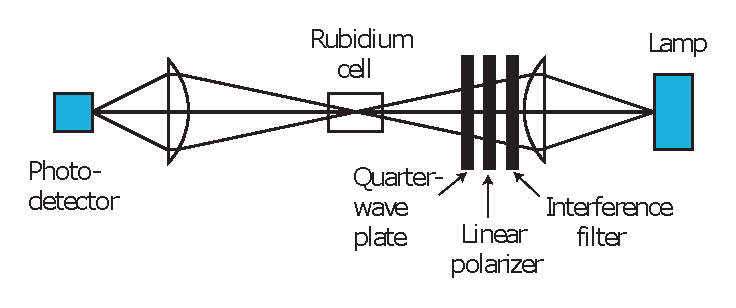
\includegraphics[width =\linewidth]{pictures/Aufbau1.pdf}
        \caption{Schematischer Aufbau des Experimentes \cite{optical_pumping}.}
        \label{fig:Aufbau1}
    \end{subfigure}
    \hfill
    \begin{subfigure}{0.48\textwidth}
        \centering
        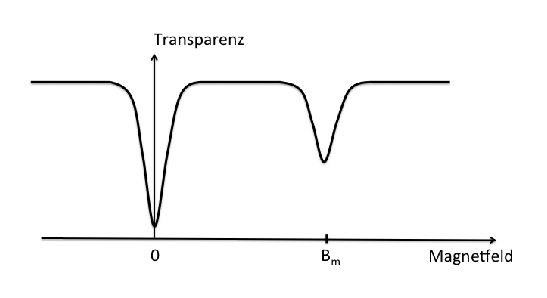
\includegraphics[width =\linewidth]{pictures/Aufspaltung1.pdf}
        \caption{Schematische Darstellung der Durchsichtigkeit der Probe \cite{v21}.}
        \label{fig:Aufspaltung1}
    \end{subfigure}
\end{figure}

In \autoref{fig:Aufbau1} ist der schematische Aufbau einer in diesem verwendeten Pumpe zu sehen.
Zunächst wird das Licht zirkular (D1) polarisiert und das  frequenzvariables Hochfrequenzmagnetfeldfeld eingeschaltet.
Hierdurch kann die Anregung des Materials besser kontrolliert werden, da die Händigkeit der Photonen bekannt ist.
Durch ständiges Pumpen kommt es dann in der Probe zur Besetzungsinversion und es kann statistisch gesehen immer weniger Licht aufgenommen werden.
Somit wird die Probe \enquote{durchsichtiger}, da das Licht nun zunehmend durch die Probe kommt.
Dies ist schematisch in \autoref{fig:Aufspaltung1} dargestellt.

% \subsection{Transiente Effekte}

% Transiente Effekte treten genau dann auf, wenn das frequenzvariables Hochfrequenzmagnetfeldfeld (RF) so justiert wird, dass es genau die Resonanzfrequenz des Systems trifft.
% Diese Resonanzfrequenz ist gegeben durch
% \begin{equation*}
%     \omega_0 = 2 \pi \nu_0 = g_\text{F} \frac{\mu_0}{h} \cdot B_0 \, .
% \end{equation*}

% Wird ein senkrechtes RF-Feld angelegt, so präzedieren die Elektronen wegen ihrem magnetischen Moment.
% Es kann gezeigt werden \cite{optical_pumping}, dass für den Resonanzfall das Verhältnis 
% \begin{align}
%   \label{eq:resonanz_perioden}
%   \frac{T_{87}}{T_{85}} &= \frac{\gamma_{85}}{\gamma_{87}}
% \end{align}
% gilt. Dabei ist $T = \frac{1}{\gamma B_\text{RF}}$ die Periode und $\gamma = g_\text{F} \frac{\mu_0}{h}$ das gyromagnetische Verhältnis.